% Chapter 2

\chapter{Theory and Motivation} % Chapter title

\label{ch:theory} % For referencing the chapter elsewhere, use \autoref{ch:examples} 
The \ac{SM} of particle physics represents all particles and interactions currently understood by the particle physics community. It is formulated using the principles of Quantum Field Theory, with the constraints of several symmetries and physical requirements to determine the rules for allowed interactions. \cite{Burgess:2007zi} Developed in the 1960s and 70s, it has been immensely successful at predicting additional particles, and has held up to many high-precision tests. Despite this success, it has several shortcomings which point to its incompleteness. Though the \ac{SM} is likely correct at the energies thus far probed, it may be missing key components that become more important at higher energies. Models supplementing the \ac{SM} with additional particles and interactions are referred to as \ac{BSM} theories. 

One possible extention of the \ac{SM} is \ac{SUSY}, a theory which applies an additional symmetry between bosons and fermions to the \ac{SM}, creating a spectrum of \ac{SUSY} particles (sparticles) which interact with the particles of the \ac{SM}. This theory motivates the search performed in \autoref{part:search}, and its theoretical appeals are discussed in this section, along with specific simplified models considered in the search. 

%----------------------------------------------------------------------------------------

\section{The Standard Model}
\label{sec:standard_model}
The \ac{SM} of particle physics describes the interactions of all of the particles currently known to exist, and consists of both matter particles and force carriers. This model has been unprecidentedly successful in predicting new particles and phenomena, including the prediction of the Higgs particle almost 50 years before its discovery in 2012, which completed the \ac{SM}. This section describes the components of the \ac{SM} and how they interact, focusing on the environment of the \ac{LHC}. 

The particles of the \ac{SM} are divided into two categories: fermions and bosons. The fermions comprise all the matter described by the \ac{SM}, and are spin-$\frac{1}{2}$ particles. The bosons, integer-spin particles, are the force carriers. They provide a mechanism to explain three of the four forces known to particle physics, with gravity still lacking a quantum formuliziation. The Higgs boson, the only spin-0 particle in the \ac{SM}, provides a mechanism for giving mass to the other particles. The full \ac{SM}, with the addition of the hypothetical graviton, is presented in \autoref{fig:sm}. 

\begin{centering}
\begin{figure}[bth]
\myfloatalign
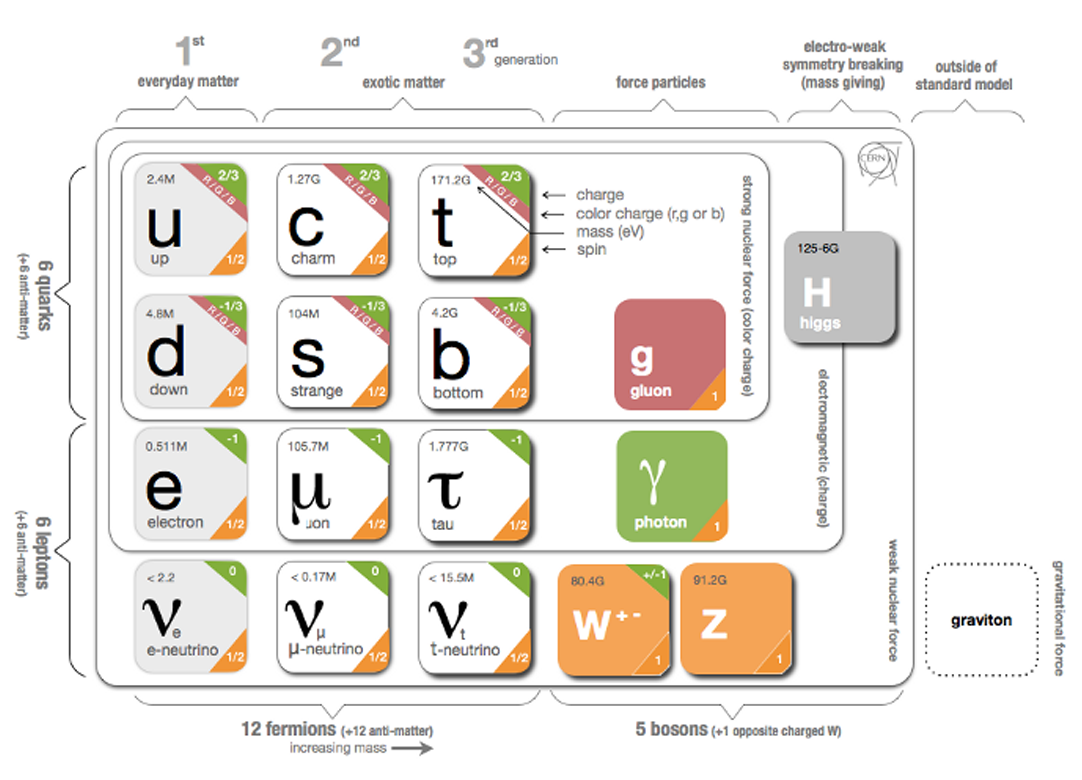
\includegraphics[width=.85\linewidth]{figures/theory/standardmodel.png}
\caption{The Standard Model of particle physics, containing all known bosons and fermions, with the addition of the hypothetical graviton. \cite{Galbraith:2012}}
\label{fig:sm}
\end{figure}
\end{centering}

\subsection{Matter}
\label{sec:matter}

The matter described by the \ac{SM} is made up of fermions, spin-$\frac{1}{2}$ particles which can be broken into two groups, quarks and leptons. The leptons all interact weakly, while the quarks additionally interact strongly. 

\subsubsection{Leptons}

Leptons, as seen in the bottom left of \autoref{fig:sm}, come in three generations, each labeled by a flavor: electron, muon, and tau. In the case of the massive leptons, these flavors are mass eigenstates, and the generations are placed in an order based on increasing mass. Each massive lepton is negatively charged and has a positively charged anti-particle. 

The three neutrinos come in the same flavors as the massive leptons, but these flavor eigenstates do not correspond exactly to mass eigenstates. As a consequence, neutrinos oscillate between flavors as they propagate through space. These oscillations are the only evidence of neutrino mass, which is bound from below by the mass splittings determined from the oscillation. Though it is still uncertain if the masses of the neutrinos follow the same hierarchy as the massive leptons, that expected ordering is slightly preferred over the inverted hierarchy. \cite{Huang:2016} 

Unlike the massive leptons, the neutrinos are uncharged, and it is not yet known whether each neutrino has a separate anti-particle, or if it is its own antiparticle. Because they are uncharged, they can only interact weakly, making them extremely difficult to detect. In the ATLAS detector, neutrinos pass through all layers undetected, and their presence can only be inferred from the non-conservation of momentum that results in the observed particles. As a consequence of their ability to evade detection, neutrinos are the least understood particles of the \ac{SM}. 

The \ac{SM} conserves lepton number, $L$, which is defined as the number of leptons minus the number of anti-leptons in a state. While this conservation is not theoretically required, its violation has not yet been observed. As a consequence of this conservation, the lightest massive lepton, the electron, is stable.

\subsubsection{Quarks}
\label{sec:quarks}

Quarks, as seen in the top left of \autoref{fig:sm}, are also charged particles that interact weakly, but are differentiated from the leptons by their strong interactions. They are also organized in three generations ordered by mass, and come in pairs of ``up-type'' and ``down-type'' quarks, named after the lightest generation. Though the up quark is lighter than the down, that rule is reversed in the subsequent two generations. Up-type quarks are charged $+\frac{2}{3}$, while the down-type quarks are charged $-\frac{1}{3}$. Quarks are also charged under the strong interaction, whose three charges are often characterized by colors: red, green, and blue. Each quark has an anti-particle with the opposite charges. 

These fractional charges and individual colors are never seen in nature because of the requirement (discussed further in \autoref{sec:strong}) that stable particle states be color-neutral. To accomplish this, quarks can create two-particle bound states called \textit{mesons} consisting of one quark and one anti-quark with the same color charge or three-particle bound states of quarks or anti-quarks with the three different color charges, which are called \textit{baryons}. The lightest color neutral state containing only quarks, the proton ($uud$), is stable. Extremely unstable bound states consisting of higher numbers of quarks can also exist, such as the pentaquark discovered in 2015 at the \ac{LHC}. \cite{Pentaquark} Collectively, these multi-quark bound states are called \textit{hadrons}. 

Like leptons, the number of quarks in a state is conserved. However, because quarks cannot exist in an isolated state, that conservation described as a conservation of baryon number ($B$) defined similarly to lepton number. Mesons, because they have one quark and one anti-quark, have $B = 0$. 

\subsection{Forces}

The fermions in the previous section interact via the electromagnetic, weak, and strong forces. In a perturbative quantum field theory, interactions via these forces are represented by mediating bosons. These force carriers interact only with particles charged with their  force's quantum numbers. The photon, for example, interacts only with electromagnetically charged particles. Gluons, mediators of the strong force, interact only with color charged particles, quarks and gluons. All fermions are weakly charged and interact with the weak force's mediators, the $W$ and $Z$ bosons. 

The formulation for each of these forces is developed by requiring that the \ac{SM} lagrangian be locally gauge invariant. \cite{Griffiths:111880} This can be accomplished by adding gauge fields to the lagrangian, whose behavior under gauge transformations cancels out the gauge dependence of the free lagrangian. However, adding a mass term for these fields reintroduces gauge dependence, so this mechanism only creates forces mediated by massless particles. 

\subsubsection{The Electromagnetic Force}

The simplest example of gauge invariance requirements generating a description of a force can be found in electromagnetism. It has one massless mediator, the photon, which interacts with all electromagnetically charged particles. What follows is a brief description of how enforcing this invariance generates a lagrangian of the same form as the classical electromagnetic lagrangian, which can be easily incorporated into the \ac{SM}. 

The particles in ~\autoref{sec:matter} are fermions, and so their free lagrangians are Dirac lagrangians and all follow the form

\begin{equation}
\mathcal{L} = i\bar{\psi}\gamma^\mu \partial_\mu\psi - m \bar{\psi}\psi . 
\end{equation}

Requiring that the free lagrangians for these particles be invariant under a $U(1)$ local gauge transformation, $e^{iq\lambda(x)}$, can be accomplished by adding a term to the lagrangian which cancels the derivative term arising from $\lambda$'s dependence on $x$: 

\begin{equation}
\mathcal{L} = i\bar{\psi}\gamma^\mu \partial_\mu\psi - m \bar{\psi}\psi - (q\bar{\psi}\gamma^\mu\psi)A_\mu
\end{equation}

where $A_\mu$ is a ``gauge field'' that transforms according to 

\begin{equation}
A_\mu \rightarrow A_\mu + \partial_\mu \lambda . 
\end{equation}

This vector field must also come with a free term, 

\begin{equation}
\mathcal{L} = -\frac{1}{16\pi}F^{\mu\nu}F_{\mu\nu} + \frac{1}{8\pi}m_A^2A^\nu A_\nu . 
\end{equation}

The mass term for this field would not itself be invariant under the transformation, but the field can simply be made massless to avoid this problem. The final lagrangian, then, is 

\begin{equation}
\mathcal{L} = i\bar{\psi}\gamma^\mu \partial_\mu\psi - m \bar{\psi}\psi -\frac{1}{16\pi}F^{\mu\nu}F_{\mu\nu} - (q\bar{\psi}\gamma^\mu\psi)A_\mu
\label{eq:l_em}
\end{equation}

which is precisely the original lagrangian with the addition of terms replicating the form of the Maxwell lagrangian. In a quantized interpretation, it describes a field that interacts with particles with non-zero electromagnetic charge $q$ via interactions with a massless spin-1 boson, the photon. 

For the purpose of succinct notation, this lagrangian is often rewritten in terms of the ``covariant derivative''

\begin{equation}
\mathcal{D}_\mu = \partial_\mu + iq\lambda A_\mu
\end{equation}

which immediately cancels the gauge dependent term created by the transformation. This mechanism is mathematically simple in the $U(1)$ case, but can be replicated for more complicated gauge transformations with perturbative approximations. 

\subsubsection{Quantum Chromodynamics}
\label{sec:strong}

\ac{QCD}, the theory desribing the strong force, can be formulated similarly to the electromagnetic force, but with a $SU(3)$ transformation replacing $U(1)$. This transformation acts on a vector of equal mass quarks, the three different colors of a given flavor. The transformation is written as follows,

\begin{equation}
\bm{\psi} \rightarrow e^{-iq\bm{\lambda}\cdot\bm{\phi}(x)}\bm{\psi}
\end{equation}

where $\bm{\phi}$ gives a vector of coefficients to be multiplied by the Gell-Man matrices, $\bm{\lambda}$. Though the math is more complicated than the $U(1)$ case in this higher dimensional rotation, the cancelation is ultimately similar. 

The main difference, corresponding to this more complicated basis of transformations, is that eight fields $A_\mu$ are required rather than the one needed in electromagnetism. These eight fields correspond to eight massless bosons, the different color states of the gluon, the carrier of the strong force.  

All together, the total lagrangian for \ac{QCD} is

\begin{equation}
\mathcal{L} = i\bar{\psi}\gamma^\mu \partial_\mu\psi - m \bar{\psi}\psi -\frac{1}{16\pi}\bm{F}^{\mu\nu}\bm{F}_{\mu\nu} - (q\bar{\psi}\gamma^\mu\psi)\bm{A}_\mu , 
\end{equation}

an equation identical in form to \autoref{eq:l_em}, with the mathematical complications of the additional fields hidden by the vector notation. In addition to that change, the covariant derivative must accomodate a vector $\bm{A}$ as well, changing only slightly to be defined as

\begin{equation}
\mathcal{D}_\mu = \partial_\mu + iq\bm{\lambda} \cdot \bm{A}_\mu .
\end{equation}

This canceling is actually only satisfied to a first order expansion of the transformation, guaranteeing its validity only for infinitesimally small $\bm{\phi}$. However, the strong coupling constant, $\alpha$, depends on the energy scale of the interaction, decreasing at higher energy scales and asymptotically increasing at low energies. \autoref{fig:alpha} shows this effect translated to distance scales, demonstrating that QCD is weak and can be considered perturbatively at small distance scales, but at large distance scales this approximation breaks down, and the colorless hadrons introduce in ~\autoref{sec:quarks} must be used to describe interactions instead. The boundary between these regimes is referred to as $\Lambda_{QCD}$. 

\begin{centering}
\begin{figure}[bth]
\myfloatalign
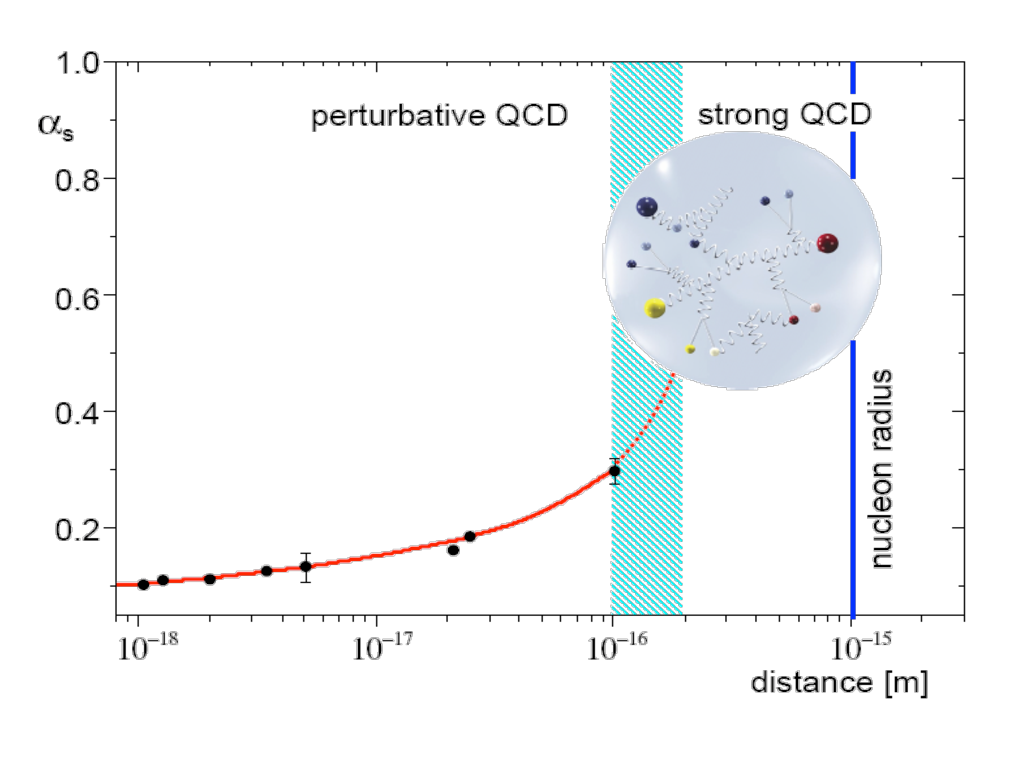
\includegraphics[width=.85\linewidth]{figures/theory/strong_coupling.png}
\caption{The running of the strong coupling constant, $\alpha$. \cite{Messchendorp:2013ysj}}
\label{fig:alpha}
\end{figure}
\end{centering}

\subsubsection{The Weak Force}

A similar process, using an $SU(2)$ gauge transformation, can produce a lagrangian that would suffice to describe the $W$ and $Z$ bosons of the \ac{SM}, if only they were massless. However, they are not, so an alternate mechanism must be used to add masses to the lagrangian. 

Before a mechanism for their masses was understood, and before they were discovered, the large mass of the $W$ and $Z$ bosons were proposed in order to unify the electromagnetic and weak forces into the electroweak force. The large masses were crucial to explain the discrepancy in the strength of the two forces. 

This unified theory resulted in a triplet, $\bm{W}$, with coupling $g_W$, and a singlet field $B$, with coupling $g'/2$. However, this electroweak symmetry is broken, and mixing between these states occurs. Rewritten in their mass basis, the more familiar electroweak force carriers are produced: $W^\pm$, two states with identical coupling, $Z^0$, and $A$, the photon field. 

\subsubsection{The Higgs Mechanism}

The reason for this symmetry breaking has to do with the final piece of the \ac{SM}, the Higgs boson. The Higgs mechanism presents an alternate way to generate a mass term, through an unexpected route. It is a scalar field, with a lagrangian 

\begin{equation}
\mathcal{L} = \frac{1}{2}(\partial_\mu\phi)(partial^\mu\phi) + \frac{1}{2}\mu^2\phi^2 - \frac{1}{4}\lambda^4\phi^4
\end{equation}

This looks very similar to the standard scalar field, but the signs on the mass and interaction terms are reversed, giving a result that looks like an imaginary mass. However, this lagrangian differs from all previously considered lagrangians in that its ground state does not occur at $\phi = 0$. Because this is a perturbative theory, its validity only holds when expanded around the ground state, which when calculated is

\begin{equation}
\phi = \pm \frac{\mu}{\lambda} . 
\end{equation}

The original lagrangian can be put in terms of $\eta$, defined as

\begin{equation}
\eta = \phi \pm \frac{\mu}{\lambda}  
\end{equation}

to read

\begin{equation}
\mathcal{L} = \frac{1}{2}(\partial_\mu\eta)(\partial^\mu\eta) - 
\end{equation}


\subsection{Phenomenology of Proton-Proton Collisions}
\label{sec:pp_collisions}

As discussed in \autoref{ch:lhc}, the \ac{LHC} collides bunches of high-energy protons, and interactions of these protons' constituent quarks produce the wide array of particles seen in the ATLAS detector. 


\subsubsection{Parton Distribution Functions}

%------------------------------------------------

\subsection{Problems in the Standard Model}
\label{sec:sm_problems}


%------------------------------------------------

\section{Supersymmetry}

\subsection{Supersymmetry Phenomenology}
\subsection{Solutions to Standard Model Problems}
\subsection{Supersymmetry Signatures in $p-p$ Collisions}
\subsubsection{Simplified Models Used in This Analysis}
\label{sec:simplified_models}

\section{Monte Carlo Generators}
\label{sec:MC_gen}